%setting document class
\documentclass[a4paper,10pt]{article}

%importing packages
\usepackage[utf8]{inputenc}
\usepackage[T1]{fontenc,url}
\usepackage[english,]{babel}
\usepackage{blindtext}
\usepackage{natbib}
\usepackage{gensymb}
\usepackage{amsmath}
\usepackage{changepage}
\usepackage{amssymb}
\usepackage{commath}
\usepackage{physics}
\usepackage{multicol}
\usepackage{float}
\usepackage{listings}
\usepackage{graphicx}
\usepackage{hyperref}
\usepackage{svg}
\usepackage{wrapfig}
\usepackage{fancyhdr}
\usepackage{color}

\definecolor{awesome}{rgb}{1.0, 0.13, 0.32}
\definecolor{mygray}{rgb}{0.5,0.5,0.5}
\definecolor{cadetgrey}{rgb}{0.57, 0.64, 0.69}

%listing customization
\lstset{ %
  backgroundcolor=\color{white},
  basicstyle=\footnotesize,        % the size of the fonts that are used for the code
  breakatwhitespace=true,         % sets if automatic breaks should only happen at whitespace
  breaklines=true,                 % sets automatic line breaking
  captionpos=b,                    % sets the caption-position to bottom
  commentstyle=\color{cadetgrey},    % comment style
  deletekeywords={...},            % if you want to delete keywords from the given language
  escapeinside={\%*}{*)},          % if you want to add LaTeX within your code
  extendedchars=true,              % lets you use non-ASCII characters; for 8-bits encodings only, does not work with UTF-8
  frame=single,	                   % adds a frame around the code
  keepspaces=true,                 % keeps spaces in text, useful for keeping indentation of code (possibly needs columns=flexible)
  keywordstyle=\color{awesome},       % keyword style
  language=c++,                 % the language of the code
  otherkeywords={...},           % if you want to add more keywords to the set
  rulecolor=\color{black},         % if not set, the frame-color may be changed on line-breaks within not-black text (e.g. comments (green here))
  showspaces=false,                % show spaces everywhere adding particular underscores; it overrides 'showstringspaces'
  showstringspaces=false,          % underline spaces within strings only
  showtabs=false,                  % show tabs within strings adding particular underscores
  stepnumber=2,                    % the step between two line-numbers. If it's 1, each line will be numbered
  stringstyle=\color{mymauve},     % string literal style
  tabsize=3,	                   % sets default tabsize to 2 spaces
}

%fixing the header 
\pagestyle{fancy}
\renewcommand{\headrulewidth}{0pt}
\fancyhf{}
\fancyhead[CO]{\textsc{asprusten \& rasmussen \& san }}
\fancyfoot[C]{\thepage}

%front page title/author setup
 \title{FYS 4150 - Computational Physics\\
 Project 1: Solving Poisson's equation in one dimension 
}
 \date{\normalsize{4. September 2018} }
 \author{
 \textsc{\small{Maren Rasmussen}}\and \textsc{\small{Markus Leira Asprusten}}\and \textsc{\small{Metin San}}
 }
 
\newcommand{\der}[2]{\frac{d #1}{d #2}}
\newcommand{\dder}[2]{\frac{d^2 #1}{d #2 ^2}}
\newcommand{\peder}[2]{\frac{\partial #1}{\partial #2}}


 %starting the document
\begin{document}
\maketitle
\begin{center}
\textsc{Abstract}
\end{center}

\begin{adjustwidth}{7mm}{7mm}

This project involves solving the one-dimensional Possion equation with dirichlet boundary conditions using two different algorithms. The first method is the tridiagonal matrix algorithm while the second is the LU decomposition. The two methods are then compared in terms of efficiency. The conclusion of the project is that a specialized version of the tridiagonal algorithm is much faster.

\end{adjustwidth}



\bigskip

\begin{center}
\textsc{1. Introduction}
\end{center}
The main goal of this project is to get familiar with the programming language c++. The focus will be directed at obtaining an understanding of vector and matrix operations with memory allocation in addition to managing library packages such as the c++ library Armadillo. 

We will address this issue by studying and solving Possion's differential equation numerically. Many of the most important differential equations in physics can be written as linear second-order differential equations. It is therefore of importance to be able to to solve these systems. 

The report starts of with a theory section where the Possion equation is introduced and discretized.  What follows is a method and algorithm section where we derive and experiment with two specific numerical algorithms which can be applied to solve the equation at hand. The first is the tridiagonal matrix algorithm, and the second is the LU-decomposition method. The more general tridiagonal matrix algorithm is further tailored to specifically deal with the Possion equation in order to increase the methods efficiency. Both algorithms are then tested at different precision levels using varying grid points. The speed and efficiency, along with the errors produced from the two methods are then presented in the results section, and further compared and discussed in the final discussion section.


\newpage


\begin{center}
\textsc{2. Theoretical Background}
\end{center}
2.1. \textbf{The Poisson Equation.} 
Poisson's equation is a classical and well known differential equation from electromagnetism. The equation describes the potential field $\Phi$ generated from a charge distribution $\rho(\textbf{r})$. For three dimensions, the equation is given by
\begin{equation}\label{eq:1}
 \nabla^2 \Phi = -4 \pi \rho(\textbf{r}),
\end{equation}
where $\nabla = $ is the Laplace operator. If both $\Phi$ and $\rho(\textbf{r})$ is spherically symmetric, the equation can be simplified to a one dimensional equation in r,
$$ \frac{1}{r^2}  \der{}{r} \left( r^2 \der{\Phi}{r} \right)= -4 \pi \rho(r).$$
By substituting $\Phi = \phi(r)/r$, we can simplify the equation even more, giving 
$$ \dder{\phi}{r} = -4\pi \rho(r). $$ 
The final equation can be written in a general form by letting $\phi \rightarrow u$ and $r \rightarrow x$, and defining the right hand side of the equation as $f$,
\begin{equation}\label{eq:2}
 - u''(x) = f(x).
\end{equation}

In this study we will assume that the source term is $f(x) = 100 e^{-10x}$ with $x \in [0,1]$. We will also assume that we have Dirichlet boundary conditions, such that $ u(0) = u(1) = 0. $ With these assumptions the equation have an exact solution on the form $u(x) = 1 - (1 - e^{-10})x - e^{-10x}$. The exact solution is of importance as it can be compared to the numerical calculation in order to verify the accuracy of our results.  \\



\noindent 2.2. \textbf{Discretization of the problem.} 
To solve the Poisson equation nummerically, we need to discretize the problem. The discretization can be done using $(n+1)$ $x$-values, so that $x \in [x_0, x_1, x_2, ..., x_n]$ with $x_0 = 0$ and $x_n = 1$, and $u(x_i) = u_i$. The $x$-values are then given as 
$$ x_i = x_0 + ih, $$
where $h = (x_n - x_0)/n$ is the step size. \\

A discretized version of $u''(x)$ can be found using Taylor expansion. We know that
\begin{align*}
u(x + h) &= u(x) + h u' + \frac{h^2}{2!} u'' + O(h^2), \\
u(x - h) &= u(x) - h u' + \frac{h^2}{2!} u'' + O(h^2). 
\end{align*} 
The $O(h^2)$-term is the remaining terms from the Taylor expansion, or the error we get by excluding these terms. By adding $u(x + h)$ and $u(x-h)$, we can derive the desired expression:
\begin{align*}
u(x + h) + u(x - h) &= 2 u(x) + \frac{2}{2!} h^2 u'' + O(h^2), \\
u''(x) &= \frac{u(x+1) + u(x-h) - 2u(x)}{h^2} + O(h^4),
\end{align*}
\begin{equation}\label{eq:3}
u'' =  \frac{u_{i+1} + u_{i-1} - 2u_i}{h^2}+ O(h^2)
\end{equation}
By excluding the rest of the terms in the Taylor expansion, and using the definition in equation \eqref{eq:2} discretized, we can define $f_i^* = f_i h^2 $. This reduces equation \eqref{eq:3} to

\begin{equation}\label{eq:4}
u_{i+1} - u_{i-1} + 2u_i = f_i^* .
\end{equation}
Inserting for specific $i$-value leaves us with a set of linear equations
\begin{align*}
-u_2 - u_0 + 2u_1 &= f_1^* , \\
-u_3 - u_1 + 2u_2 &= f_2^*,\\
\vdots \\
-v_n - v_{n-2} + 2v_{n-1} &= f_{n-1}^*. \\
\end{align*}
This set of equations can also be represented in terms of matrices. The LHS of the equation can be splitted up into the product of a matrix $\mathbf{\hat{A}}$ and a vector $\mathbf{\hat{u}}$

$$
\mathbf{\hat{A}} \mathbf{\hat{u}} = 
\begin{bmatrix}
                           2& -1& 0 &\dots   & \dots &0 \\
                           -1 & 2 & -1 &0 &\dots &\dots \\
                           & \dots   & \dots &\dots   &\dots & \dots \\
                           0&\dots   &  &-1 &2& -1 \\
                           0&\dots    &  & 0  &-1 & 2 \\
\end{bmatrix}
\begin{bmatrix}
	 u_1\\
          u_2 \\
   	\vdots \\
 	u_{n-1}
\end{bmatrix},
$$
and the RHS as a vector $\mathbf{\hat{f}}$
$$ \mathbf{\hat{f}} =  
\begin{bmatrix}
	 f_1^*\\
          f_2^* \\
   	\vdots \\
 	f_{n-1}^* 
\end{bmatrix}. $$
This means that the set of equations can be written as a linear algebra problem on the form
$$ \mathbf{\hat{A}} \mathbf{\hat{u}} = \mathbf{\hat{f}}.$$

\bigskip

\begin{center}
\textsc{3. Algorithm \& Implementation }
\end{center}
With the problem now formulated in terms of linear algebra, the next step is to solve it. We will tackle this problem through the implementation of two algorithms. The first is the Tridiagonal matrix algorithm, also known as the Thomas algorithm. The second is the LU-decomposition algorithm. 
\bigskip

\noindent 3.1. \textbf{Tridiagonal Matrix Algorithm.} This algorithm is a simplified form of Gaussian elimination which can be used to solve tridiagonal systems of equations. In the general case, a tridiagonal system of $n$ unknowns can be represented as 

\begin{equation}\label{eq:5}
a_i u_{i-1} + b_i u_i +c_i u_{i+1} = b_i,
\end{equation}
where $a_1 = c_1 = 0$. Or in matrix representation as $\mathbf{\hat{A}} \mathbf{\hat{u}} = \mathbf{\hat{f}}$. We spot that this corresponds to our linear algebra problem with Possion's Equation. Written out in the $4 \cross 4$ case, this becomes
\begin{equation}\label{eq:6}
\begin{bmatrix}
b_1 & c_1 & 0 & 0 \\
a_2& b_2 & c_2 & 0 \\
0 & a_3 & b_3 & c_3 \\
0 & 0 & a_4 & b_4 
\end{bmatrix}
\begin{bmatrix}
u_1 \\
u_2 \\
u_3 \\
u_4
\end{bmatrix}
=
\begin{bmatrix}
f_1\\
f_2\\
f_3\\
f_4
\end{bmatrix}.
\end{equation}
The algorithm is quite simple and consists of mainly two steps, a forward substitution and a backwards substitution. The forward substitution reduces the tridiagonal matrix $\mathbf{\hat{A}}$ to an upper tridiagonal matrix. This is achieved through Gaussian elimination. We want to get rid of the $a_i$ terms located on the lower secondary diagonal. We perform the following row reduction on both sides of the equation
\[
\begin{bmatrix}
b_1 & c_1 & 0 & 0 \\
a_2& b_2 & c_2 & 0 \\
0 & a_3 & b_3 & c_3 \\
0 & 0 & a_4 & b_4 
\end{bmatrix}
\xrightarrow{\text{II} - \frac{a_2}{b_1}\text{I}}
\begin{bmatrix}
b_1 & c_1 & 0 & 0 \\
0& \tilde{b_2}  & c_2 & 0 \\
0 & a_3 & b_3 & c_3 \\
0 & 0 & a_4 & b_4 
\end{bmatrix}, \qquad
\begin{bmatrix}
f_1\\
f_2\\
f_3\\
f_4
\end{bmatrix}
\xrightarrow{\text{II} - \frac{a_2}{b_1}\text{I}}
\begin{bmatrix}
f_1\\
\tilde{f_2}\\
f_3\\
f_4
\end{bmatrix}
\]
where $\tilde{b_2} = b_2 - a_2c_1/b_1$, and $\tilde{f_2} = f_2 - f_1a_2/b_1$, and II and I denotes the row 1 and 2 in the $\mathbf{\hat{A}}$. Similarly for the second row

\[
\begin{bmatrix}
b_1 & c_1 & 0 & 0 \\
0& \tilde{b_2}  & c_2 & 0 \\
0 & a_3 & b_3 & c_3 \\
0 & 0 & a_4 & b_4 
\end{bmatrix}
\xrightarrow{\text{III} - \frac{a_3}{b_2}\text{II}}
\begin{bmatrix}
b_1 & c_1 & 0 & 0 \\
0& \tilde{b_2}  & c_2 & 0 \\
0 & 0 & \tilde{b_3} & c_3 \\
0 & 0 & a_4 & b_4 
\end{bmatrix}, \qquad
\begin{bmatrix}
f_1\\
\tilde{f_2}\\
f_3\\
f_4
\end{bmatrix}
\xrightarrow{\text{III} - \frac{a_3}{b_2}\text{II}}
\begin{bmatrix}
f_1\\
\tilde{f_2}\\
\tilde{f_3}\\
f_4
\end{bmatrix}
\]
where $\tilde{b_3} = b_3 - a_3c_2/b_2$, and $\tilde{f_3} = f_3 - f_2a_3/b_2$. Finally we compute the last row reduction

\[
\begin{bmatrix}
b_1 & c_1 & 0 & 0 \\
0& \tilde{b_2}  & c_2 & 0 \\
0 & 0 & \tilde{b_3} & c_3 \\
0 & 0 & a_4 & b_4 
\end{bmatrix}
\xrightarrow{\text{IIII} - \frac{a_4}{b_3}\text{III}}
\begin{bmatrix}
b_1 & c_1 & 0 & 0 \\
0& \tilde{b_2}  & c_2 & 0 \\
0 & 0 & \tilde{b_3} & c_3 \\
0 & 0 & 0 & \tilde{b_4} 
\end{bmatrix}, \qquad
\begin{bmatrix}
f_1\\
\tilde{f_2}\\
\tilde{f_3}\\
f_4
\end{bmatrix}
\xrightarrow{\text{III} - \frac{a_3}{b_2}\text{II}}
\begin{bmatrix}
f_1\\
\tilde{f_2}\\
\tilde{f_3}\\
\tilde{f_4}
\end{bmatrix}
\]

where $\tilde{b_4} = b_4 - a_4c_3/b_3$, and $\tilde{f_4} = f_4 - f_3a_4/b_3$. 

\newpage

We are then left with the row reduced form of the set of equations $\tilde{\mathbf{A}}\mathbf{\hat{u}} = \tilde{\mathbf{f}}$, or in matrix notation

\begin{equation}\label{eq:7}
\begin{bmatrix}
b_1 & c_1 & 0 & 0 \\
0& \tilde{b_2}  & c_2 & 0 \\
0 & 0 & \tilde{b_3} & c_3 \\
0 & 0 & 0 & \tilde{b_4} 
\end{bmatrix} \begin{bmatrix}
u_1\\
u_2\\
u_3\\
u_4
\end{bmatrix} = \begin{bmatrix}
f_1\\
\tilde{f_2}\\
\tilde{f_3}\\
\tilde{f_4}
\end{bmatrix}.
\end{equation}
If one takes a closer look at the steps which we carried out, one notices the following pattern for $\tilde{b}$ and $\tilde{d}$. These can be generally expressed as

\begin{equation}\label{eq:8}
\tilde{b_i} = b_i - \frac{a_i c_{i-1}}{\tilde{b}_{i-1}}, \qquad 
\tilde{f_i} = f_i - \frac{a_i \tilde{f}_{i-1}}{\tilde{b}_{i-1}}, \qquad i \in [2,4],
\end{equation}
where $b_1 = \tilde{b_1}$ and $f_1 = \tilde{f}$. In general for a $(n \cross n)$ matrix we would have $i \in [2,n]$. 
The forward substitution has been implemented in the following way in c++:

\lstinputlisting[language=c++, firstline=67, lastline=74]{../1b/problem_b.cpp}
Note that instead of allocating memory for a seperate $\tilde{b}$ array, we have rather reused the b array. We also compute $a_i / \tilde{b}_{i-1}$ at the start of the loop which saves us a FLOP as it appears in both the expression for $\tilde{b}$ and $\tilde{f}$.

The last part of the tridiagonal algorithm is the backwards substitution. By setting up the set of equations in \eqref{eq:7}, we are able to solve each of these for their respective solution $u_i$. The first equation along with its solution is then
\[
\tilde{b}_1 u_1 + c_1 u_2 = \tilde{f_1} \qquad \rightarrow \qquad u_1 = \frac{\tilde{f}_1 - c_1 u_2}{\tilde{b_1}},
\]
where we have used that $b_1 = \tilde{b}_1$. Similarly for the second and the third rows
\[
\tilde{b}_2 u_2 + c_2 u_3 = \tilde{f_2} \qquad \rightarrow \qquad u_2 = \frac{\tilde{f}_2 - c_2 u_3}{\tilde{b_2}},
\]
\[
\tilde{b}_3 u_3 + c_3 u_4 = \tilde{f_3} \qquad \rightarrow \qquad u_3 = \frac{\tilde{f}_3 - c_3 u_4}{\tilde{b_3}}.
\]
For the final row, we simply get
\[
\tilde{b}_4 u_4 = \tilde{f}_4 \qquad \rightarrow \qquad u_4 = \frac{\tilde{f_4}}{\tilde{b}_4}.
\]
This is a result of the chosen dirichlet boundary conditions. Again we notice the solution $u_i$ follows the following pattern
\begin{equation}\label{eq:9}
u_i = \frac{\tilde{f}_i - c_i u_{i+1}}{\tilde{b}_i}.
\end{equation}
\newpage
This is implemented in the code as
\lstinputlisting[language=c++, firstline=76, lastline=81]{../1b/problem_b.cpp}
where we see that the last term has been computed separately as it differs from the general algorithm. Prior to these two code snippets are the allocation of memory to the different vectors that are to be used in the algorithm. The code displayed here has used classic c++ memory allocation. We have however also created corresponding armadillo code to every program which can be found on the Github together with the classical code.

In general one of the most important aspects of any algorithm is its efficiency. The tridiagonal matrix algorithm is known to be a relatively fast algorithm as it only uses three diagonal vectors to represent the entire $(n \cross n)$ matrix which severely reduces the number of floating points operations (FLOPS) required to solve the set of equations. We will assume that addition, subtraction, multiplication and division all counts as FLOPS. In reality, division operations are said to be "heavier" than the other three operations. The forward substitution method requires 6 FLOPS for each iteration, and it is computed $(n-2)$ times which results in a total of $6(n-2)$ FLOPS. The backward substitution requires $3(n-2) +1 $ FLOPS where the $+1$ term comes from the definition of the last term, which has to be computed just once.

\bigskip

\noindent 3.1.1 \textbf{Optimizing the Tridiagonal Matrix Algorithm.}
The number of floating point operations in the algorithm can be severely reduced if we specialize it for our special case with the Poisson equation. Since we are only interested in the tridiagonal matrix which resulted from the discretization of the second derivative, we can use the precomputed matrix $\mathbf{\hat{A}}$. This allows us to rewrite the expressions for the forward and backwards substitution. If one inserts for the constant $a_i =  c_i = -1$ and $b_i = 2$ into equations \eqref{eq:8} and \eqref{eq:9}, we find that we can in fact rewrite these into the form

\begin{equation}\label{eq:10}
\tilde{b}_i = 2 - \frac{1}{\tilde{b}_{i-1}} = \frac{i+1}{i},
\end{equation}
\begin{equation}\label{eq:11}
\tilde{f}_i = f_i + \frac{(i-1)\tilde{f}_{i-1}}{i},
\end{equation}
\begin{equation}\label{eq:12}
u_{i} = \frac{i}{i+1}(\tilde{f}_{i} +u_{i+1}).
\end{equation}
Now, since the diagonal elements $\tilde{b}_i$ can be precomputed as they only depend on $i$, we can move this calculation outside of the main algorithm. Further, we spot that we can rewrite (?) in terms of $\tilde{b}_{i-1} = i/(i-1) $, to the form
\begin{equation}\label{eq:13}
\tilde{f}_i = f_i + \frac{\tilde{f}_{i-1}}{\tilde{b}_{i-1}}
\end{equation}
Which has now been reduced to 2 FLOPS down from 3. Similarly we rewrite the (?) in terms of $\tilde{b}_i$ to the from
\begin{equation}\label{eq:14}
u_i = \frac{\tilde{f}_i + u_{i+1}}{\tilde{b}_i},
\end{equation}
which has now also been reduced to 2 FLOPS down from 3. 
The new specialized algorithm is implemented in the
 following way
\lstinputlisting[language=c++, firstline=66, lastline=77]{../1c/problem_c.cpp}
The total number of FLOPS is then reduced to $4(n-2) + 1$ operation, which is half that of the general algorithm. 

Finally we are interested in finding out how much the numerical solution deviates from the analytic. The following equation gives us the relative error $\epsilon_i$ in the data set, where $i = 1, ...,n$

\begin{equation}\label{eq:15}
\epsilon_i = \log_{10} \left( \abs{\frac{u_i - v_i}{v_i}}, \right)
\end{equation}
where $u_i$ is the numerically computed solution and $v_i$ is the exact analytic solution. The relative error $\epsilon_i$ can then be computed for different number of grid points. 

\bigskip

\begin{center}
\textsc{4. Results}
\end{center}
4.1. \textbf{The General Tridiagonal Algorithm.} As previously mentioned, the general tridiagonal matrix algorithm can solve problems for matrices of $(n \cross n)$. We have tested the algorithm for $n = 10$, $n = 100$, and  $n = 1000$. Together with the numerical solution, we also compute the exact solution mentioned in 2.1 with corresponding grid points. 

The results are produced by compiling and executing the c++ program \textit{problem\_b.cpp} with the commandline arguments $1$ $-1$ $2$ $-1$. The first argument reads in number of grid points and is calculated by $n = 10^i$ where $i$ is the commandline input. The next three arguments fills the diagonals of the tridiagonal matrix, which in this case becomes $a_i = c_i  = -1$ and $b_i = 2$ which correspond to the discretized second derivative matrix. The result for the $n= 10$ can be seen in figure \ref{fig:1}, $n = 100$ in figure \ref{fig:2}, and $n=1000$ in figure \ref{fig:3}.

\begin{figure}[h]
  \centering
  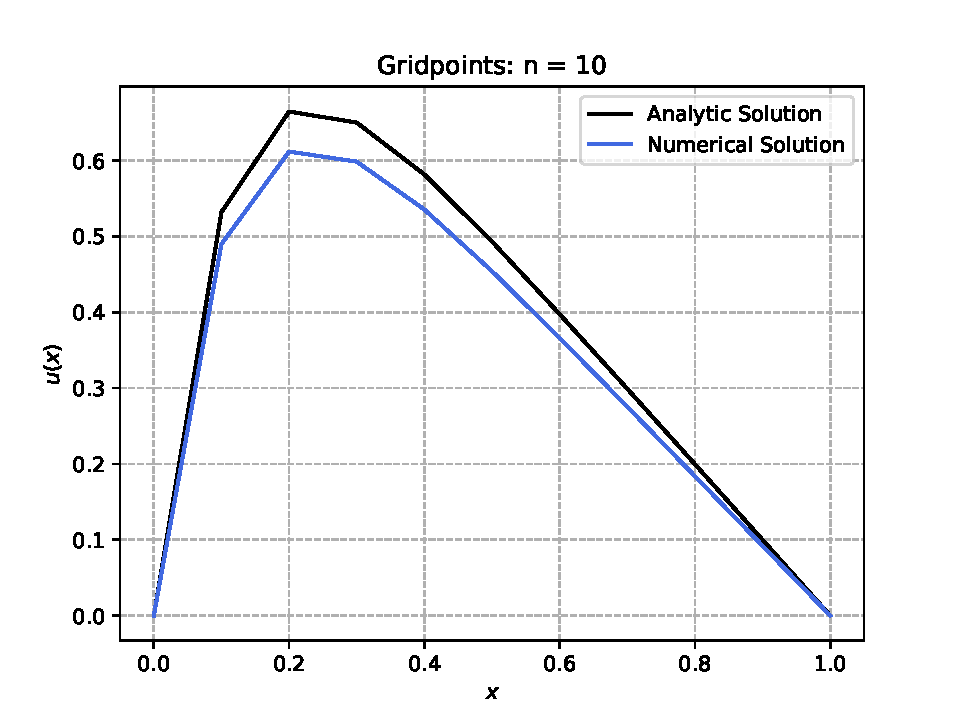
\includegraphics[width=0.9\linewidth]{figures/fig_10_b.pdf}
  \caption{Numerical and analytic solution to Poisson's equation for $n = 10$ grid points. }
  \label{fig:1}
\end{figure}

In figure \ref{fig:1} we see that the both solutions have the same shape but the numerical one converges to $x=1$ from below the analytic solution. The low number of grid points results in a non smooth curve for both the analytic and numerical solution. The Numerical solution ends up with a lower amplitude compared to the exact solution.

For the $n = 100$ case seen in figure \ref{fig:2}, we see that the numerical solution lies nearly perfectly on top of the analytic one. For a simple 100 integration points, the algorithm seems to accurately reproduce the exact solution of the Poisson equation.



\begin{figure}[h]
  \centering
  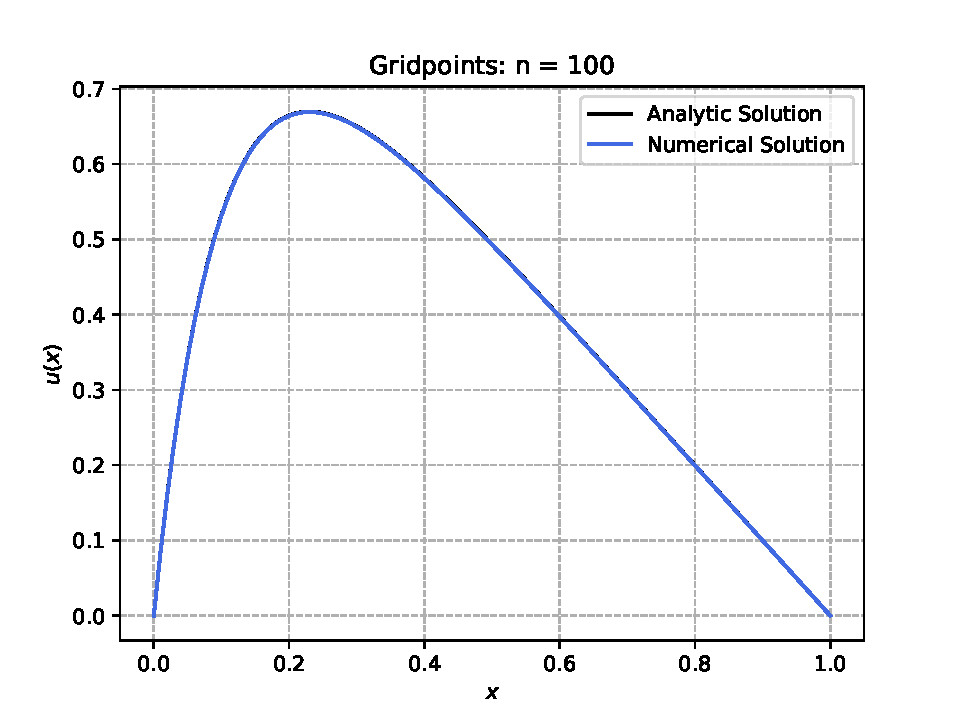
\includegraphics[width=0.9\linewidth]{figures/fig_100_b.pdf}
  \caption{Numerical and analytic solution to Poisson's equation for $n = 100$ grid points.}
  \label{fig:2}
\end{figure}


\begin{figure}[h]
  \centering
  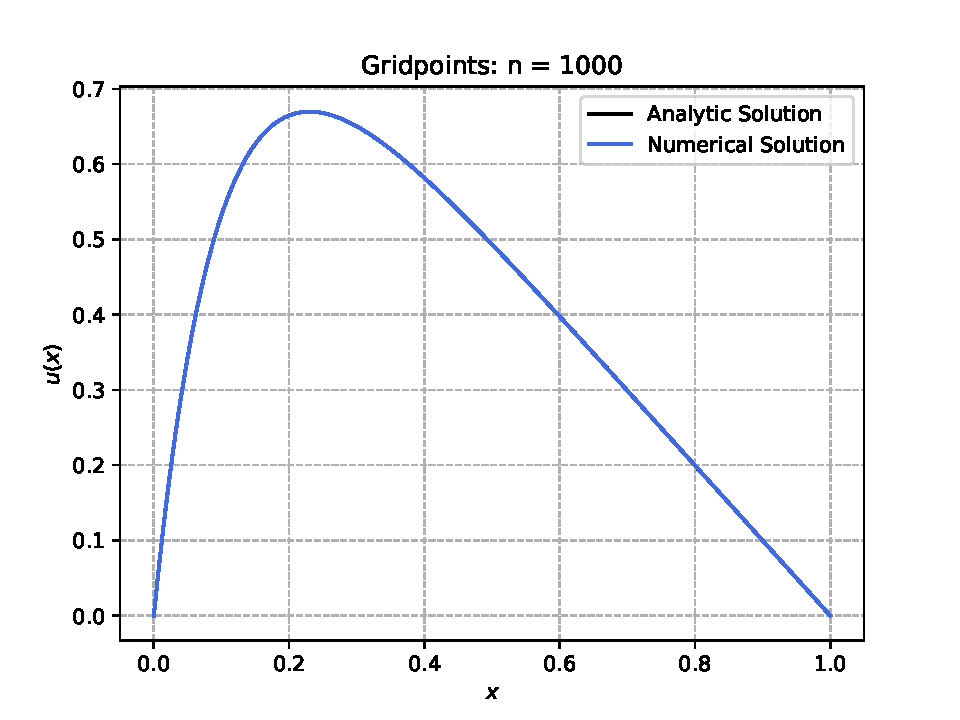
\includegraphics[width=0.9\linewidth]{figures/fig_1000_b.pdf}
  \caption{Numerical and analytic solution to Poisson's equation for $n = 1000$ grid points.}
  \label{fig:3}
\end{figure}

For the third and final precision test at $n = 1000$ seen in figure \ref{fig:3} the numerical solution is indistinguishable from the analytic one. These results suggest that our algorithm works as intended.

\bigskip

\noindent 4.2. \textbf{Special Tridiagonal Algorithm.}
The results produced by the special tridiagonal algorithm are the same as the once for the general algorithm, as was to be expected. The specialized algorithms only objective was to reduce the number of floating point operations and therefore cut the computation time of the calculation. 

\noindent 4.3 \textbf{Execution time.}
The efficiency of the algorithms is compared by extracting the execution time for each of the algorithms separately. The execution time should be proportional to the number of FLOPS required in the algorithm. The following results has been found using a MacBook Pro (Early 2015) to run the program. The program has been executed 10 times in rapid succession collecting each run time. These are then used to find an average executing time. The run time results can be seen in figure \ref{fig:5}. 

For the tridiagonal algorithm, we find that that the specialized version has a faster run time than the general one. By taking the ratio of the time averages we find that it the execution time was reduced by $20.16\%$. This is a marginal improvement in the algorithms efficiency. However, one would likely expect a run time reduction by as much as $50\%$ as the number of FLOPS was halved in the specialized version of the algorithm. 

\noindent 4.4 \textbf{Relative Error.}
Having computed the relative error for $n = 10, 100, 1000, ..., 10^7$ grid points, we can extract the maximum value of the error for each set of grid points. Max$[\epsilon_i]$ is then plotted as a function if the grid points. The result is seen in figure \ref{fig:4}.

\begin{figure}[h]
  \centering
  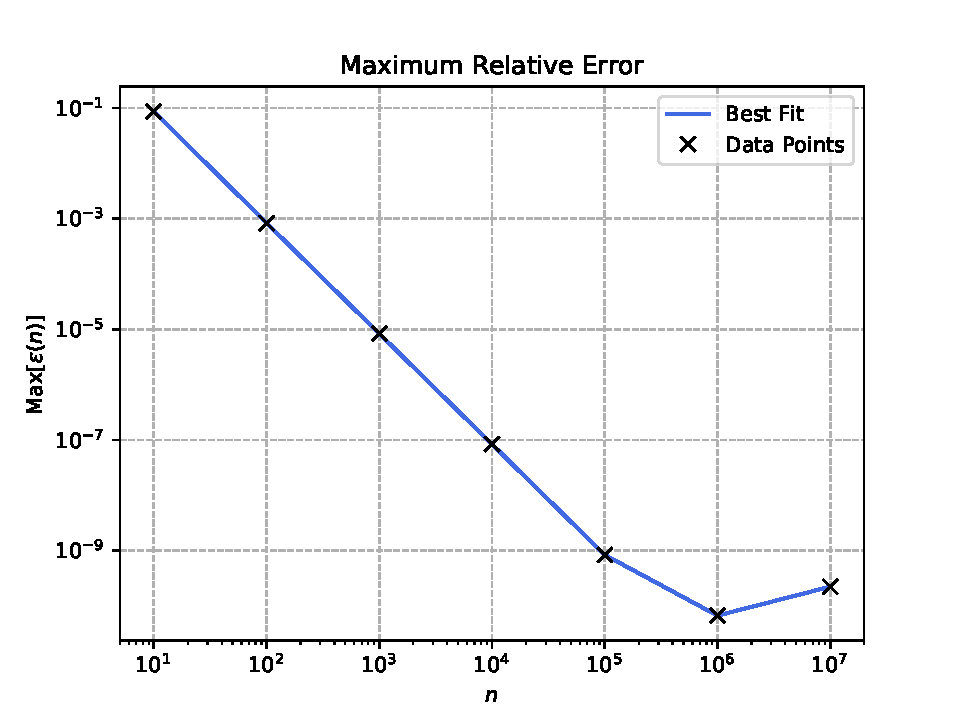
\includegraphics[width=0.9\linewidth]{figures/rel_error_plot.pdf}
  \caption{Maximum relative error as a function of grid points.}
  \label{fig:4}
\end{figure}

We see that the relative error decreases linearly with increasing number of grid points, which is expected. However, once we reach $n > 10^6$ grid points, the error starts to increase again. 



\begin{table}[]  \label{fig:5}
\begin{tabular}{lll}
\hline
General Algorithm  & Special Algorithm & LU-Decomposition \\
\hline
0.030738           & 0.023905          &                  \\
0.028017           & 0.024106          &                  \\
0.028026           & 0.024124          &                  \\
0.028299           & 0.023557          &                  \\
0.028742           & 0.024067          &                  \\
0.028511           & 0.023537          &                  \\
0.028791           & 0.02406           &                  \\
0.028829           & 0.024148          &                  \\
0.028296           & 0.023556          &                  \\
0.028575           & 0.023642          &                  \\
                   &                   &                  \\\hline
Average Time Spent &                   &                  \\
\hline
0.0286824          & 0.0238702         &                 
\end{tabular}
\end{table}


\end{document}